\documentclass[border=4pt]{standalone}
\usepackage{fontspec}
\setmainfont{DMSans9pt}[Path=../../fonts/, Extension=.ttf, UprightFont=*-Regular, BoldFont=*-Bold, ItalicFont=*-Italic, BoldItalicFont=*-BoldItalic]
\setsansfont{DMSans9pt}[Path=../../fonts/, Extension=.ttf, UprightFont=*-Regular, BoldFont=*-Bold, ItalicFont=*-Italic, BoldItalicFont=*-BoldItalic]
\usepackage{amsmath,amssymb,xcolor}
\usepackage{tikz}
\usetikzlibrary{arrows.meta,positioning,shapes.geometric,shapes.misc,fit,backgrounds,calc,decorations.pathreplacing,shadows}
\definecolor{cTwo}{HTML}{4C72B0}
\definecolor{cOne}{HTML}{DD8452}
\definecolor{cDetr}{HTML}{55A868}
\definecolor{cOvd}{HTML}{8172B3}
\definecolor{cAgent}{HTML}{C44E52}
\definecolor{cEdge}{HTML}{937860}
\definecolor{cApp}{HTML}{DA8BC3}
\definecolor{cData}{HTML}{4C9BB0}

\makeatletter
\def\refmap#1#2{\expandafter\def\csname rm@#1\endcsname{#2}}
\def\rm@ref#1{\csname rm@#1\endcsname}
\renewcommand{\ref}{\@ifstar\rm@ref\rm@ref}
\renewcommand{\eqref}[1]{(\csname rm@#1\endcsname)}
\makeatother

\refmap{eq:ciou}{10}\refmap{eq:detector}{1}\refmap{eq:dfl}{11}\refmap{eq:giou}{9}\refmap{eq:glip}{17}\refmap{eq:grpo}{20}\refmap{eq:infonce}{15}\refmap{eq:mllm-box}{19}\refmap{eq:ovd}{2}\refmap{eq:reparam}{18}\refmap{eq:roialign}{6}\refmap{eq:rpn}{5}\refmap{eq:siglip}{16}\refmap{eq:tal}{8}\refmap{sec:agentic}{5}\refmap{sec:closed}{3}\refmap{sec:manufacturing}{7.1}\refmap{sec:mllm-direct}{5.1}\refmap{sec:mllm-rl}{5.2}\refmap{sec:mllm-tools}{5.3}\refmap{sec:ovd}{4}\refmap{sec:ovd-distill}{4.2}\refmap{sec:ovd-grounding}{4.3}\refmap{sec:ovd-owl}{4.4}\refmap{sec:ovd-rt}{4.5}\refmap{sec:ovd-unified}{4.6}\refmap{sec:twostage}{3.1}\refmap{sec:vlfound}{4.1}\refmap{sec:yolo}{3.3}\refmap{tab:yolo}{4}
%% ---------- illustrative scene thumbnails (drawn, not photographs); origin = lower-left, size 2.4 x 1.7
\definecolor{pcbG}{HTML}{2E7D4F}\definecolor{pcbD}{HTML}{1F5A39}\definecolor{chipK}{HTML}{2B2B2B}
\definecolor{soil}{HTML}{8B6B4A}\definecolor{soilD}{HTML}{6E5238}\definecolor{crop}{HTML}{6BB04A}\definecolor{weed}{HTML}{3E7C2A}
\definecolor{belt}{HTML}{5A5F66}\definecolor{carton}{HTML}{C9A46A}\definecolor{cartonD}{HTML}{A9844C}\definecolor{pallet}{HTML}{9C7A4F}
\tikzset{bx/.style={draw=#1, line width=0.8pt}, bxl/.style={fill=#1, text=white, font=\fontsize{4.2}{4.2}\selectfont\bfseries, inner sep=0.6pt, anchor=south west}}
% PCB: chips, pads, one solder bridge
\newcommand{\scenePCB}{%
  \fill[pcbG, rounded corners=1pt] (0,0) rectangle (2.4,1.7);
  \foreach \y in {0.25,0.55,0.85,1.15,1.45}{\draw[pcbD, line width=0.35pt] (0.05,\y) -- (2.35,\y);}
  \fill[chipK] (0.25,0.75) rectangle (0.95,1.4);
  \foreach \x in {0.32,0.47,0.62,0.77,0.89}{\fill[gray!60] (\x-0.03,0.66) rectangle (\x+0.03,0.75); \fill[gray!60] (\x-0.03,1.4) rectangle (\x+0.03,1.49);}
  \fill[chipK] (1.35,0.2) rectangle (2.15,0.7);
  \foreach \x in {1.45,1.65,1.85,2.05}{\fill[gray!60] (\x-0.04,0.7) rectangle (\x+0.04,0.8);}
  \fill[gray!70] (1.7,1.05) circle (0.07); \fill[gray!70] (1.95,1.05) circle (0.07); \fill[gray!70] (2.2,1.05) circle (0.07);
  \fill[gray!75] (1.7,1.0) rectangle (1.95,1.1); % bridge between pads
}
% Field: soil rows with crops and weeds
\newcommand{\sceneField}{%
  \fill[soil, rounded corners=1pt] (0,0) rectangle (2.4,1.7);
  \foreach \y in {0.35,0.85,1.35}{\fill[soilD] (0.05,\y-0.06) rectangle (2.35,\y+0.06);}
  \foreach \x/\y in {0.3/0.35,0.8/0.35,1.3/0.35,1.8/0.35,0.3/0.85,0.8/0.85,1.8/0.85,2.2/0.85,0.55/1.35,1.05/1.35,1.55/1.35,2.05/1.35}{%
    \fill[crop] (\x,\y) ellipse (0.11 and 0.07); \fill[crop] (\x,\y+0.05) ellipse (0.05 and 0.1);}
  \foreach \x/\y in {1.3/0.85,0.6/0.6}{\foreach \a in {0,60,...,300}{\fill[weed, rotate around={\a:(\x,\y)}] (\x+0.07,\y) ellipse (0.07 and 0.025);}}
}
% Warehouse: belt with cartons and a pallet stack
\newcommand{\sceneWarehouse}{%
  \fill[gray!15, rounded corners=1pt] (0,0) rectangle (2.4,1.7);
  \fill[belt] (0,0.15) rectangle (2.4,0.45);
  \foreach \x in {0.1,0.5,...,2.3}{\draw[gray!50, line width=0.3pt] (\x,0.15) -- (\x,0.45);}
  \fill[carton] (0.2,0.45) rectangle (0.75,0.85); \draw[cartonD] (0.475,0.45) -- (0.475,0.85);
  \fill[carton] (1.0,0.45) rectangle (1.4,0.75); \draw[cartonD] (1.2,0.45) -- (1.2,0.75);
  \fill[pallet] (1.6,0.55) rectangle (2.3,0.65);
  \fill[carton] (1.62,0.65) rectangle (1.95,0.95); \fill[carton] (1.97,0.65) rectangle (2.28,0.95); \fill[carton] (1.75,0.95) rectangle (2.15,1.25);
  \draw[cartonD] (1.62,0.65) rectangle (1.95,0.95); \draw[cartonD] (1.97,0.65) rectangle (2.28,0.95); \draw[cartonD] (1.75,0.95) rectangle (2.15,1.25);
}
% Metal surface with scratch and dent
\newcommand{\sceneSurface}{%
  \shade[left color=gray!35, right color=gray!15, rounded corners=1pt] (0,0) rectangle (2.4,1.7);
  \foreach \i in {1,...,14}{\draw[gray!45, line width=0.2pt] (0.05,0.1*\i) -- (2.35,0.1*\i+0.03);}
  \draw[gray!80!black, line width=0.6pt] (0.4,1.25) .. controls (0.8,1.15) and (1.0,1.05) .. (1.35,0.95);
  \fill[gray!65] (1.8,0.45) ellipse (0.16 and 0.1);
}

\begin{document}
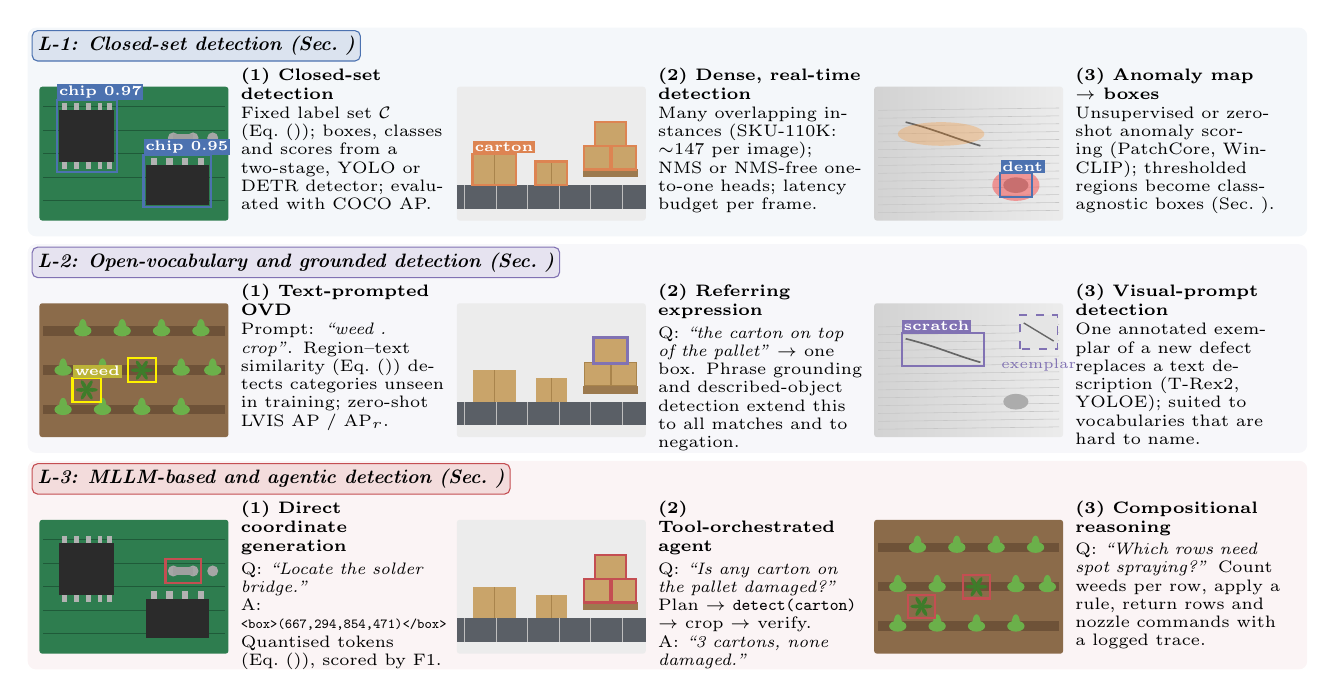
\begin{tikzpicture}[
  ptitle/.style={font=\fontsize{6.2}{7}\selectfont\bfseries\hyphenpenalty10000\exhyphenpenalty10000\relax, anchor=north west, inner sep=0pt, text width=2.6cm, align=left},
  ptext/.style={font=\fontsize{5.6}{6.6}\selectfont, anchor=north west, text width=2.6cm, align=left, inner sep=0pt},
  lvl/.style={draw=#1, fill=#1!20, rounded corners=2pt, font=\fontsize{6.8}{7}\selectfont\bfseries\itshape, inner sep=2pt, anchor=north west},
  qa/.style={text=#1},
]
\def\PW{5.3}
\newcommand{\panel}[5]{% #1 x, #2 y, #3 scene+overlay, #4 title, #5 text
  \begin{scope}[shift={(#1,#2)}]
    \begin{scope}[shift={(0,-1.95)}] #3 \end{scope}
    \node[ptitle] (pt) at (2.55,0) {#4};
    \node[ptext] at ([yshift=-0.08cm]pt.south west) {#5};
  \end{scope}}
% ---------------- row backgrounds
\foreach \y/\c/\t in {0/cTwo/{L-1: Closed-set detection (Sec.~\ref*{sec:closed})},-2.75/cOvd/{L-2: Open-vocabulary and grounded detection (Sec.~\ref*{sec:ovd})},-5.5/cAgent/{L-3: MLLM-based and agentic detection (Sec.~\ref*{sec:agentic})}}{
  \fill[\c!6, rounded corners=3pt] (-0.15,\y+0.05) rectangle (16.1,\y-2.6);
  \node[lvl=\c] at (-0.1,\y+0.02) {\t};
}
% ================= L-1
\panel{0}{-0.45}{\scenePCB
   \draw[bx=cTwo] (0.22,0.62) rectangle (0.98,1.53); \node[bxl=cTwo] at (0.22,1.53) {chip 0.97};
   \draw[bx=cTwo] (1.32,0.17) rectangle (2.18,0.83); \node[bxl=cTwo] at (1.32,0.83) {chip 0.95};}
  {(1) Closed-set detection}
  {Fixed label set $\mathcal{C}$ (Eq.~(\ref*{eq:detector})); boxes, classes and scores from a two-stage, YOLO or DETR detector; evaluated with COCO AP.}
\panel{\PW}{-0.45}{\sceneWarehouse
   \foreach \a/\b/\c/\d in {0.2/0.45/0.75/0.85,1.0/0.45/1.4/0.75,1.62/0.65/1.95/0.95,1.97/0.65/2.28/0.95,1.75/0.95/2.15/1.25}{\draw[bx=cOne] (\a,\b) rectangle (\c,\d);}
   \node[bxl=cOne] at (0.2,0.85) {carton};}
  {(2) Dense, real-time detection}
  {Many overlapping instances (SKU-110K: ${\sim}$147 per image); NMS or NMS-free one-to-one heads; latency budget per frame.}
\panel{2*\PW}{-0.45}{\sceneSurface
   \fill[red, opacity=0.35] (1.8,0.45) ellipse (0.3 and 0.2); \fill[orange, opacity=0.25] (0.85,1.1) ellipse (0.55 and 0.15);
   \draw[bx=cTwo] (1.6,0.3) rectangle (2.0,0.6); \node[bxl=cTwo] at (1.6,0.6) {dent};}
  {(3) Anomaly map $\rightarrow$ boxes}
  {Unsupervised or zero-shot anomaly scoring (PatchCore, WinCLIP); thresholded regions become class-agnostic boxes (Sec.~\ref*{sec:manufacturing}).}
% ================= L-2
\panel{0}{-3.2}{\sceneField
   \draw[bx=yellow] (1.12,0.7) rectangle (1.48,1.0); \draw[bx=yellow] (0.42,0.45) rectangle (0.78,0.75);
   \node[bxl=yellow!70!black] at (0.42,0.75) {weed};}
  {(1) Text-prompted OVD}
  {Prompt: \textit{``weed . crop''}. Region--text similarity (Eq.~(\ref*{eq:ovd})) detects categories unseen in training; zero-shot LVIS AP / AP$_r$.}
\panel{\PW}{-3.2}{\sceneWarehouse
   \draw[bx=cOvd, line width=1.1pt] (1.73,0.93) rectangle (2.17,1.27);}
  {(2) Referring expression}
  {Q: \textit{``the carton on top of the pallet''} $\rightarrow$ one box. Phrase grounding and described-object detection extend this to all matches and to negation.}
\panel{2*\PW}{-3.2}{\sceneSurface
   \draw[bx=cOvd] (0.35,0.9) rectangle (1.4,1.32); \node[bxl=cOvd] at (0.35,1.32) {scratch};
   \fill[gray!20] (1.85,1.12) rectangle (2.33,1.55); \draw[gray!80!black, line width=0.5pt] (1.9,1.45) -- (2.28,1.22); \draw[cOvd, dashed, line width=0.6pt] (1.85,1.12) rectangle (2.33,1.55); \node[font=\fontsize{4}{4}\selectfont, text=cOvd, anchor=north] at (2.09,1.12) {exemplar};}
  {(3) Visual-prompt detection}
  {One annotated exemplar of a new defect replaces a text description (T-Rex2, YOLOE); suited to vocabularies that are hard to name.}
% ================= L-3
\panel{0}{-5.95}{\scenePCB
   \draw[bx=cAgent] (1.6,0.9) rectangle (2.05,1.2);}
  {(1) Direct coordinate generation}
  {Q: \textit{``Locate the solder bridge.''}\\ A: \texttt{\fontsize{5}{6}\selectfont<box>(667,294,854,471)</box>}\\ Quantised tokens (Eq.~(\ref*{eq:mllm-box})), scored by F1.}
\panel{\PW}{-5.95}{\sceneWarehouse
   \foreach \a/\b/\c/\d in {1.62/0.65/1.95/0.95,1.97/0.65/2.28/0.95,1.75/0.95/2.15/1.25}{\draw[bx=cAgent] (\a,\b) rectangle (\c,\d);}}
  {(2) Tool-orchestrated agent}
  {Q: \textit{``Is any carton on the pallet damaged?''} Plan $\rightarrow$ \texttt{detect(carton)} $\rightarrow$ crop $\rightarrow$ verify.\\ A: \textit{``3 cartons, none damaged.''}}
\panel{2*\PW}{-5.95}{\sceneField
   \foreach \x/\y in {1.3/0.85,0.6/0.6}{\draw[bx=cAgent] (\x-0.17,\y-0.15) rectangle (\x+0.17,\y+0.15);}}
  {(3) Compositional reasoning}
  {Q: \textit{``Which rows need spot spraying?''} Count weeds per row, apply a rule, return rows and nozzle commands with a logged trace.}
\end{tikzpicture}

\end{document}
